\documentclass{beamer}
\usetheme{default}
%\usetheme{Boadilla}
\usepackage[english]{babel}
\usepackage[T1]{fontenc}
\usepackage[utf8]{inputenc}
\usepackage{times}
\parindent0em

\usepackage{graphicx}
\usepackage{float}
\inputencoding{utf8}
\usepackage{multicol}
\usepackage{vwcol} 
\usepackage{color}
\definecolor{links}{HTML}{2A1B81}
\hypersetup{colorlinks,linkcolor=,urlcolor=links}
\usepackage{listings}

\definecolor{keywords}{RGB}{255,0,90}
\definecolor{comments}{RGB}{0,0,113}
\definecolor{red}{RGB}{160,0,0}
\definecolor{green}{RGB}{0,150,0}
 
\lstset{language=Python, 
        basicstyle=\ttfamily\small, 
        keywordstyle=\color{keywords},
        commentstyle=\color{comments},
        stringstyle=\color{red},
        showstringspaces=false,
        identifierstyle=\color{green},
        procnamekeys={def,class}}


\begin{document}

\title[Group Project]{Simple Course Management System}
\subtitle{Python - Django - Postgres}
\author{Antigravity - Chris Papke, Jimmy Pardey, \\Thomas Watkin, Stefanie Fritz}
\date{\today}

\begin{frame}[plain]
\titlepage
\end{frame}

{
\usebackgroundtemplate{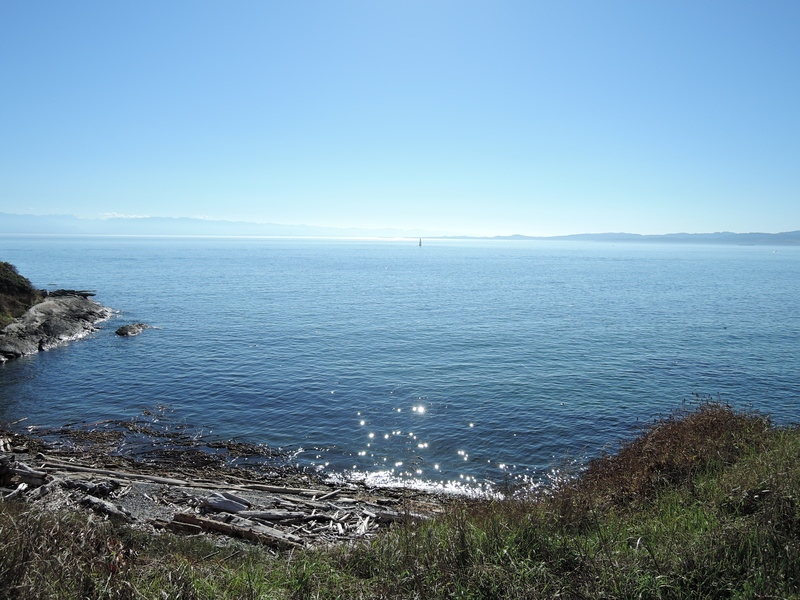
\includegraphics[width=\paperwidth]{picture.jpg}}%
\begin{frame}[fragile]
\frametitle{Replace with Real Picture}

\begin{center}
	DEMO!
\end{center}

\end{frame}
}

\section{Python}
\begin{frame}[fragile]
\frametitle{Python example}

\begin{lstlisting}
def hello(name):
    print 'Hello', name
 
if __name__=='__main__':
    hello('Me')   
\end{lstlisting}
\end{frame}


\end{document}